\documentclass[12pt]{article}


\usepackage{charter}
\usepackage{fullpage}
\usepackage[colorlinks=false]{hyperref}
\usepackage{ifthen}
\usepackage{comment}
\usepackage[title,titletoc]{appendix}
\usepackage{pagecolor}
\usepackage{amsmath}
\usepackage{amsfonts}
%\usepackage[normalem]{ulem}
\usepackage{siunitx}
\usepackage{amsthm}
\sisetup{per=slash, load=abbr}
\usepackage{paralist}
\usepackage{pgfplots}
\usetikzlibrary{positioning}
\usetikzlibrary{fit}
\usetikzlibrary{snakes}
\usetikzlibrary{shapes.geometric}
\usetikzlibrary{patterns}
\usetikzlibrary{shapes,arrows,chains}
\usepgfplotslibrary{patchplots,colormaps}
\usetikzlibrary{calc}
\usetikzlibrary{positioning, fit}
\usetikzlibrary{backgrounds}
\usetikzlibrary{intersections}

\newcommand{\whitepaper}[1]{\begin{center}\fbox{\parbox{0.75\textwidth}{{\small
#1}}}\end{center}}

\newcommand{\pcolor}{violet!25}

\usepackage{setspace}
\usepackage{algorithm2e}
\bibliographystyle{ieeetr}

\usepackage{geometry}
\geometry{left=3cm,right=3cm,top=1.6cm,bottom=3cm,headheight=0pt,headsep=1.5em}
\usepackage{fancyhdr}
\pagestyle{fancy}
\chead{
\includegraphics[scale=0.2]{../common/Nebulas.png}}  %在此处插入logo.pdf图片 图片靠左
\lhead{} % 页眉中间位置内容
\rhead{}
\usepackage{expl3}
\ExplSyntaxOn
\newcommand\latinabbrev[1]{
  \peek_meaning:NTF . {% Same as \@ifnextchar
    #1\@}%
  { \peek_catcode:NTF a {% Check whether next char has same catcode as \'a, i.e., is a letter
      #1.\@ }%
    {#1.\@}}}
\ExplSyntaxOff

%Omit final dot from each def.
\def\eg{\latinabbrev{e.g}}
\def\etal{\latinabbrev{et al}}
\def\etc{\latinabbrev{etc}}
\def\ie{\latinabbrev{i.e}}
\newcommand{\dapp}{DApp\xspace}

%\setlength{\topskip}{1em}

\usepackage{indentfirst}


\newcommand{\reffig}[1]{Fig.~\ref{#1}}
\newcommand{\refsec}[1]{~\S~\ref{#1}}


%\setlength{\parindent}{2.1em}
%\setlength{\parskip}{0.3\baselineskip}
%\newcommand{\nrcore}{Core Nebulas Rank}
%\newcommand{\nrext}{Extended Nebulas Ranks}
\newcommand{\nr}{\Gamma}
%\newcommand{\dom}{{\; \texttt{dom}\;}}

\onehalfspacing

\newtheorem{property}{Property}
\newtheorem{corollary}{Corollary}
%\addbibresource{reference.bib}

\begin{document}
\pagestyle{empty}
%\renewcommand{\nomname}{术语表(按首字母排序)}
%\renewcommand{\baselinestretch}{1.5}

\pagecolor{\pcolor}

\begin{titlepage}
  \begin{center}
    \vspace*{5.5cm}
    
\includegraphics[scale=0.5]{../common/Nebulas.png}
    \vspace{0.5cm}


    \textbf{\huge{Mauve Paper: Developer Incentive Protocol}}

    \vspace{0.5cm}
    Nebulas Research
    \vfill
    October 2018\\
    Version:1.0.0
    \textbf{}
  \end{center}

\end{titlepage}
\setcounter{page}{0}
%\thispagestyle{empty}
\tableofcontents
\newpage
\setcounter{page}{1}
\pagestyle{fancy}
\vspace*{0.01cm}
\section{Introduction}

Generally, developers develop applications on some application platforms (like
Windows\footnote{\url{https://www.microsoft.com/en-us/windows}}, Linux\footnote{\url{https://en.wikipedia.org/wiki/Linux}},
macOS\footnote{\url{https://en.wikipedia.org/wiki/MacOS}},
iOS\footnote{\url{https://en.wikipedia.org/wiki/IOS}},
Android\footnote{\url{https://en.wikipedia.org/wiki/Android}} \etc) and
benefit from their applications in traditional software development industry.
The way to get the benefits varies for different developers, including but not
limited to salaries paid by software enterprises, revenue by selling the
application licenses or displaying advertises in their applications.

However, the enterprises who build the application platforms also benefit
from the applications, while the benefits are not shared with the developers.
Let's take the operating system as an example here: a UI/UX designer wants to use \texttt{Sketch},
as we know that the application only works on \texttt{macOS} device, so besides
paying for the application itself, the designer needs to pay Apple\footnote{\url{https://en.wikipedia.org/wiki/Apple_Inc.}}
for the device  to use the application. Apparently, Apple benefits from such user while
Apple does not share the benefits with the \texttt{Sketch} developers.
Another similar example is that users have to pay Apple or
Microsoft\footnote{\url{https://en.wikipedia.org/wiki/Microsoft}} to use
AutoCAD\footnote{\url{https://en.wikipedia.org/wiki/AutoCAD}}. In such cases,
the key factor that users choose a platform is whether the platform
supports required applications for users. In other words, high-quality
applications are critical to the development of an application platform. Based on the above considerations,  application platforms ignore the interests of developers, to a certain extent, infringing the interests of developers.

In the blockchain industry, the interests of \dapp(Decentralized Application) developers are ignored by platforms  as  well.
 In 2004, Ethereum community proposed ``Smart Contract'',
which extended blockchains' ability from peer-to-peer
cryptocurrency networks to decentralized application platforms. However, in comparison with traditional centralized development industry, the ways of obtaining revenue for developers have no significant difference --- decentralized application developers still can not benefit
 from the increment of the blockchain system's value.


Generally speaking,  new-block rewards represent incremental values of the blockchain system and the distribution of such rewards determines the incentive direction of the decentralize system. In our opinion, a blockchain system's incremental value essentially comes from the implicit values from users' data, which should be distributed to all contributed parties, including \dapp deveploers. However, what we see in practice is that, in most PoW blockchain systems, represented by Bitcoin, new-block rewards are distributed to miner nodes; In PoS (proof of stake) based blockchain systems, new-blocks rewards are assigned to  stake holders. Along with it, the interests of \dapp developers are somewhat infringed.


Conceptually, a \dapp is a set of smart contracts with a series of specific
functionalities, while a smart contract is a computer protocol intended to
digitally facilitate, verify, or enforce the negotiation or performance of a
contract. Smart contracts allow the performance of credible transactions
without third
parties\footnote{\url{https://en.wikipedia.org/wiki/Smart\_contract}}.

From the technical architecture's point of view, most \dapp usually uses smart contracts as the back-end, while using common front-end technologies and its interactions. {\dapp}s' forms can be either a traditional PC client, mobile applications or web applications.

We believe that the relationship among decentralized application platforms, \dapp developers and \dapp users is mutually reinforcing and symbiotic. Firstly, the emergence of decentralized application platforms enlarges the group of blockchain developers. More and more developers try to develop {\dapp}s that meet different requirements and benefit from the development of {\dapp}s. Secondly, \dapp developers provide a rich variety of {\dapp}s, expanding the application scenarios of the blockchain, and bringing more incremental users to the blockchain. Finally, \dapp users drive the continuous optimization and upgrade of decentralized application platforms, increasing the mobility of tokens on the decentralized application platform, making the whole blockchain system develop.

It should be noted that the developers described here only refer to developers on the decentralized application platform, not specifically the Nebulas developers, nor the developers of the blockchain system itself.
Notice that we mean \dapp developers instead of Nebulas \dapp developers or
blockchain system developers. Thus, we shall use developers short for \dapp
developers without ambiguity. Also, a \dapp developer may be a stake holder.
He may benefit from being a stake holder and that benefit is not considered
as sharing the increase value of blockchains. The interests of being a developer can still be ignored or infringed.


It's inappropriate to directly distribute a platform's increased value to
corresponding application developers. One the one hand, the revenue is owned by
centralized organizations, like an enterprise, and application developers have
no chance to know the details of or participate in the sharing of revenues. Second, it
is difficult to quantify each developer's contribution to the growth of
application platforms so the fairness of the reward mechanism is hard to be guaranteed. Fortunately, this situation can be changed in blockchain
industry since each invocation to smart contracts by each user is
publicly recorded on blockchain. Thus, it is possible to \emph{reward or incentive each \dapp developer by
quantifying each \dapp's contribution}.

An ideal incentive mechanism should satisfy some basic properties:
\begin{itemize}

\item Fairness: the protocol should maintain objectivity when rewarding developers, that is, every {\dapp}s should be equally treated and their usages are evaluated veritably, even there are some potential manipulations.

\item Effectiveness: the reward should reflect user preference, that is, the {\dapp}s with high reward are ones that frequented by active users while the {\dapp}s with low or no reward are unwelcome.
\end{itemize}


In this paper, we propose Developer Incentive Protocol (DIP), which aims at rewarding and incentivizing  developers, enabling the developers to benefit from the development of the decentralized application platform. Naturally, an ideal developer incentive protocol does not exist since the users' evaluations to  {\dapp}s are subjective and multi-dimensioned. So the DIP introduced in the paper still has space for improvement. However, the balance in this mauve paper is innovative, that is, under the premise of guaranteeing the interests of \dapp developers, in terms of resistance to manipulation, we make the greatest efforts.

DIP is designed based on the existing Nebulas Rank
(NR)~\cite{Nebulasyellowpaper} and it benefits from some good features of NR\@.
Intuitively, DApp evaluation is reduced to a voting process in DIP\@.

An invocation from a certain user is treated as a vote and user's voting
capacity is a function of his/her NR\@. The developers will get the rewards from the system eventually, according to the voting results.

Besides giving the theoretical model of Developer Incentive Protocol, we also
analyze the properties against manipulations and illustrate the
implementation of DIP, such as, how to adjust and update DIP\@, which specify the direction of the actual landing of the DIP.

\whitepaper{

Special Hint: As the mauve paper dedicated to discussing Developer Incentive
Protocol, Mauve Paper: Developer Incentive Protocal greatly upgrades and expands the relevant chapters of the Nebula Technology White Paper~\cite{Nebulaswhitepaper}(version 1.02 released in April 2018). Compared with the conceptual demonstration one year ago, after a year of in-depth thinking and practical verification, we are confident and able to design more rigorous algorithms and provide clear solutions or directions for more practical details of the Nebulas Incentive Protocal.

}

\section{Background}
\label{sec:background}
The DIP given by this mauve paper referred  lots of related works and also extended our previous results. Here we introduce the related works, which play a significant role for the  reference and guidance of this mauve paper.

\subsection{DApp's Developer Incentive}
As for as we know, currently, no decentralized platform on blockchain offers a long-term effective incentive mechanism for DApp developers. As a representation of blockchain 2.0, Ethereum makes a breakthrough to involve turing-complete smart contracts. A number of DApps emerge on Ethereum, including game, gambling, crowd sourcing, credit and many other types. In particular, the CryptoKitties in the late 2017 and Fomo 3D in 2018 attract most attentions, which once cause network congestions. 

Actually, like the two famous DApps, most DApps gain utilities only by charging fees to users, unable to benefit from the increment of Ethereum's value or the rewards for new blocks. 

With the lack of the incentive of developer, the application scenarios of DApps has also been affected to a certain extent. For example, implicitly, free DApps may be aborted due to the difficulty for getting a return. As a result, the quantity, quality and diversity of DApps are affected. In contrast, a fair and effective mechanism for incentivizing developers enables developers to focus on the development of DApps, which further promotes the prosperity and sustainable development of the whole blockchain ecosystem.

To a certain extent, many emerging blockchain systems recognize the necessity of incentive mechanism for building blockchain ecosystems. For example, in Nebulas Incentive Program, more than 6781 DApps have been generated and a large number of excellent development teams can go to the front desk and obtain high investments. 

Along with it, other public blockchains also launched short-term incentive programs based on centralized management. Such incentive programs mainly aims to publicize to the community with official evaluations taking a major role, without long-term sustainability.


\subsection{Nebulas Rank}
Nebulas Rank (NR)~\cite{Nebulasyellowpaper} gives each account's contribution to the total economic output and has nice properties against manipulations. In particular, Nebulas Rank introduces the Wilbur function, which has the following properties: 

\begin{property}
	\label{prop:one}
	For any two positive variables $x_1$,$x_2$, the sum of their functions is less than the function of their sum. 
	%对于任意输入$x$,将其拆分后的计算函数之和小于原计算函数。
\end{property}
\begin{align}
	f(x_1+x_2)>f(x_1)+f(x_2) \quad x_1>0,x_2>0
\end{align}
\begin{property}
	\label{prop:two}
	For any two positive variables $x_1$,$x_2$, when they tend to infinity, the sum of their functions tends to the function of their sum. 
\end{property}

\begin{align}
	\lim\limits_{x_1 \to \infty, x_2\to \infty} f(x_1+x_2) = f(x_1) + f(x_2)\quad x_1>0, x_2>0
\end{align}
\noindent As the basis of NR, the two properties also offer nice properties for DIP against manipulations. 

\subsection{Voting Mechanism}
As mentioned earlier, in DIP, the process that users use DApps can be regarded as a process that voters vote for DApps. The later's incentive mechanism is similar to ranking algorithms. 

About voting mechanism and ranking algorithm, there are lots of related work in various fields, which we have referred and show examples as follows. 

One of the most famous results is the Arrow's Theorem, which shows that no ranking algorithm can simultaneously satisfy Pareto Efficiency, i.e., the ranking results satisfies the majority's interest, non-dictatorship and independent of irrelevant alternatives, i.e. the relative ranking of two candidates is not affected by any third candidate. 

The result implies that no ranking algorithm can cover everything. So the DIP in this mauve paper will focus on more important and well-known attributes. 

In the real life, there are a lot of scenarios requiring ranking algorithms. A typical and related example is the buyers' impressions to sellers (merchant) on Amazon and Taobao. Sellers with higher reputations will be given better display slots thus obtain more attentions and higher click-through rates (CTRs). In particular, such e-commerce platforms exist similar problems like Sybil attack, i.e., creating fake transactions or buy over buyers to obtain 5-star evaluations. 

For now, even these centralized platforms mostly rely on machine learning to distinguish normal and fake users~\cite{mukherjee2013spotting,jindal2008opinion,yoo2009comparison}. However, practical results show that such methods are not ideal. ~\cite{ott2011finding} points out that even artificial identifications can not effectively distinguish such accounts. ~\cite{cai2016mechanism} gives an algorithm that eliminates the incentive of such manipulations, based on mechanism design. Although its model is different form us, it can used as a significant reference.

~\cite{salihefendic2010hacker} introduces the ranking algorithm for postings in a network community, which combines the users' votes and time declining. ~\cite{salihefendic2010reddit} introduces the ranking algorithm for postings in Reddit, which involves the situation where users can vote in the negative. 
~\cite{miller2009how} introduced Reddit's ranking algorithm for the comments, taking the confidence interval into account.
IMDB ~\cite {IMDB} introduces the idea of Bayesian Model Averaging to film rankings, which can narrow the gap between different films due to the number of voters.

Because of properties against manipulation in NR, the DIP designed in this mauve paper can distinguish normal users and fake users more clearly. Therefore, the emphasis of this mauve paper is to transfer users' NR values to DApps' ranking scores through interactive behaviors.



\section{开发者激励模型}
开发者激励协议,DIP,包括两个环节:DApp评分以及开发者激励分配。

首先对于构建一个优秀的排名系统,其意义在于为第三方开发者提供了方便且高效的应用推广平台,同时也能为用户提供可信的推荐环境。正如目前移动端的App Store平台,优秀App在排行榜上拥有更显著的位置进而能受到更多用户的关注,而用户能通过排行榜上直接获取高质量的App无疑能提高其体验。更进一步地,App排名也可以应用于关键词搜索中,类似于搜索引擎和电商平台中的搜索功能,与关键词相关的候选DApp将按排名分顺序展示在搜索结果中,增加用户对搜索结果的满意程度。

另一方面,正如我们在第二章所提到的,DIP旨在为优秀DApp的开发者提供奖励,这进一步增加了开发者设计优秀DApp的动机,对整个生态的开发起到了促进作用。因此DIP第二个环节则是根据DApp评分排名提出公平的激励分配策略。

\subsection{模型表示}
\label{subsection:parameters}
首先我们给出DIP模型中涉及的符号表示。
\begin{itemize}
	\item $\mathcal{A}=\{a_1,a_2,...,a_m\}$表示所有参与此阶段评选的投票用户的集合,注意的是只有在一定时间内调用过任何DApp的外部账户(External Owned Account)才会被定义为投票用户。同时期所有用户集合表示为$\mathcal{A}^*=\{a_1,a_2,...,a_m,a_{m+1},...,a_k\}$。
	\item $\mathcal{D}=\{d_1,...,d_n\}$表示此阶段所有DApp的集合。
	\item $e_{ij},i=1,2,...,m, j=1,2,...,n$表示在一定时间内用户$a_i$对DApp $d_j$的总调用次数。鉴于区块链系统所具有的公开性,去中心化等特性,因此DIP评分模型和传统中心化的应用商城评分系统有所不同。简单地说,DIP将在去中心化系统中基于用户调用智能合约行为DApp评分的功能,具体描述见下一节。
	\item $\nr_i, i=1,2,...,m$表示参与评选的用户$a_i$在此阶段的平均NR值。\cite{Nabulasyellowpaper}中已经证明NR值是衡量一个用户的有效价值尺度,故我们也把其用作DIP模型中用于决定用户投票权重的重要指标。
	\item $\nr_{ij}, i=1,2,...,m,j=1,2,...,n$表示用户$a_i$对DApp $d_j$的分贡献值。可以理解为$a_i$愿意为$d_j$投的票数。%在我们的模型里由$a_i$对所有DApp的调用次数决定。
	\item $score_j, j=1,2,...,n$,表示DApp $d_j$的排名分,由该DApp从用户获得的所有分贡献值决定。直观地,排名分的高低直接决定了DApp在排行榜上所处的位置。%一种对排名分最简单的定义方式为所有分贡献值相加。而我们的模型采取了更合理的排名分计算方式。
	\item $M$表示星云团队用于给与开发者奖励总奖金池。实际发放的奖励总额会根据该阶段社区参与度来适当进行加权调整。
	\item $u_j, j=1,2,...,n$,表示DApp $d_j$开发者最终获得的奖励,这个奖励由奖励总额以及所有Dapp的排名分共同决定。%生活中常见的评奖方式通常具有凹函数性质,例如第一名10000元,第二名5000元,第三名2000元。我们的奖励函数具有同样性质且具有更高的可扩展性。
\end{itemize}

\begin{figure}
	\centering
 %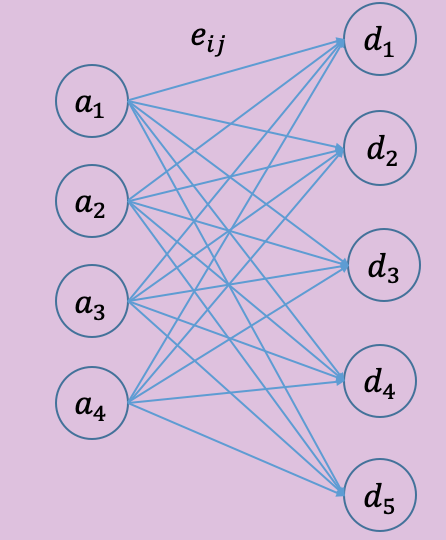
\includegraphics[width = 0.4\textwidth]{../common/m2.png}
  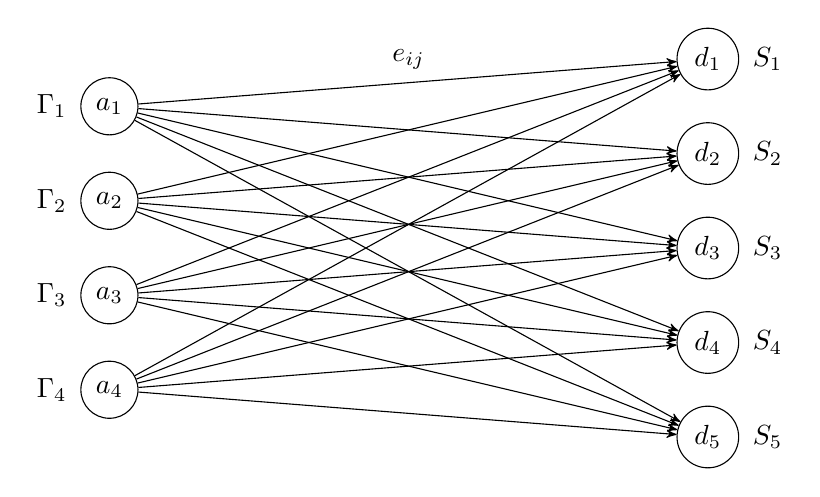
\begin{tikzpicture}
\pgfmathsetmacro{\XTD}{3.8}
\pgfmathsetmacro{\YTD}{1.2}

\tikzset{
  node/.style={draw, circle, on grid, align=center, minimum height=2ex},
}

\node[node] (d1) at (\XTD, 2*\YTD) {$d_1$};
\node[node] (d2) at (\XTD, \YTD) {$d_2$};
\node[node] (d3) at (\XTD, 0) {$d_3$};
\node[node] (d4) at (\XTD, -1*\YTD) {$d_4$};
\node[node] (d5) at (\XTD, -2*\YTD) {$d_5$};

\node [right=0.05 of d1] {${S}_{1}$};
\node [right=0.05 of d2] {${S}_{2}$};
\node [right=0.05 of d3] {${S}_{3}$};
\node [right=0.05 of d4] {${S}_{4}$};
\node [right=0.05 of d5] {${S}_{5}$};

\node[node] (a1) at (-\XTD, 1.5*\YTD) {$a_1$};
\node[node] (a2) at (-\XTD, 0.5*\YTD) {$a_2$};
\node[node] (a3) at (-\XTD, -0.5*\YTD) {$a_3$};
\node[node] (a4) at (-\XTD, -1.5*\YTD) {$a_4$};

\node [left=0.05 of a1] {${\nr}_{1}$};
\node [left=0.05 of a2] {${\nr}_{2}$};
\node [left=0.05 of a3] {${\nr}_{3}$};
\node [left=0.05 of a4] {${\nr}_{4}$};

\draw[->, >=stealth'] (a1) to (d1);
\draw[->, >=stealth'] (a1) to (d2);
\draw[->, >=stealth'] (a1) to (d3);
\draw[->, >=stealth'] (a1) to (d4);
\draw[->, >=stealth'] (a1) to (d5);

\draw[->, >=stealth'] (a2) to (d1);
\draw[->, >=stealth'] (a2) to (d2);
\draw[->, >=stealth'] (a2) to (d3);
\draw[->, >=stealth'] (a2) to (d4);
\draw[->, >=stealth'] (a2) to (d5);

\draw[->, >=stealth'] (a3) to (d1);
\draw[->, >=stealth'] (a3) to (d2);
\draw[->, >=stealth'] (a3) to (d3);
\draw[->, >=stealth'] (a3) to (d4);
\draw[->, >=stealth'] (a3) to (d5);

\draw[->, >=stealth'] (a4) to (d1);
\draw[->, >=stealth'] (a4) to (d2);
\draw[->, >=stealth'] (a4) to (d3);
\draw[->, >=stealth'] (a4) to (d4);
\draw[->, >=stealth'] (a4) to (d5);

\node at (0, 2*\YTD) {$e_{ij}$};

\end{tikzpicture}

\caption{用户与DApp间的交互 \label{fig:interact}}
\end{figure}

综上,用户和DApp之间的交互可以用图\ref{fig:interact}中的二分图来表示。

\subsection{投票行为}
在中心化的App Store中,系统会记录App的下载量等信息,后者也是应用评分的主要参考因素之一。而在区块链场景下,用户对于应用的使用会直接反应在调用合约地址行为上,例如表现为一段时间内用户$a_i$对DApp $dj$的总调用次数$e_{ij}$。DIP通过用户调用行为作为用户的投票数据来源,相比传统的下载量信息具有如下优点:
\begin{itemize}
	\item 用户调用智能合约行为记录在链上,很难篡改,相比中心化的下载量统计方式更加公开透明;
	\item 调用次数相比下载量信息更加细粒度,下载量只能记录用户一次性行为,而优秀的DApp应具有用户黏性,因此调用次数更能反映用户的真实使用情况。
\end{itemize}

实际上用户在调用智能合约时,还有其他信息可获取,例如调用智能合约过程中的gas消耗以及在调用过程中可能涉及到的资金交互,而DIP没有采取上述两者作为参考依据。

首先,用户每次调用智能合约gas消耗量是与智能合约内部的执行语句相关,而后者与DApp本身质量没有任何相关性。同时,目前星云系统中智能合约调用gas消耗开销平均只有$10^{-8}$数量级的NAS,可以忽略不计。

%所花费的gas费用以及向合约地址支付的费用不会被排名算法考虑进去,即用户支付更多的钱无法提高其投票效用。前者是因为在

而不考虑调用合约过程中资金转移的原因在于有效防作弊手段的缺失。直觉上来说,用户在使用DApp过程中愿意额外支付token确实能提高该DApp的被认同度。但实际情况下,这笔交易中token的最终流向存在以下三种可能。
\begin{enumerate}
\item Token最终归智能合约即DApp开发者所有。这种情况可以认为用户自愿付出这些钱给DApp,但此时DApp开发者相当于已经从中获益,再提高其排名获取额外奖励的意义不大。

\item DApp机制设计需要资金流通,例如博彩类DApp,其与用户之间存在大量资金交互。这是一种正常现象,此时用户与DApp的资金交互的动机主要在于用户希望通过这类交易获利,而并不能反应DApp本身质量,不应据此提高DApp排名。

\item DApp开发者承诺所有为其投入的钱最终会返还到用户手里。这本质上是一种作弊手段,而据此提高DApp排名将会助长此种作弊手段。
\end{enumerate}

实际上在不解析智能合约代码的情况下也无法判断用户和智能合约地址的资金交互属于上述哪一种情况,并且上述任何一种情况都存在不介入排名的理由,故DIP最终的算法独立于用户和DApp间的资金交互。

在DIP模型中,$a_i \in \mathcal{A}$本质上是一个账户地址,正如\cite{Nabulasyellowpaper}所提到的,一个用户实际上可以控制多个账户地址,由于建立新的账户地址是没有成本的,用户可以伪造出多个受他控制的地址进行投票,进行女巫攻击(Sybil Attack)。类似地,DApp开发者也可以选择将自己的Dapp分成多个地址,即将一个DApp拆分成多个低质量的DApp,并且获得这些DApp的总奖励。同时一个DApp开发者也可以线下收买用户为他进行投票。

在设计DIP时,我们分析了上述作弊行为,并且设计了对应的解决方案。关于DIP抗作弊分析详见章节\ref{section:properties}。


%但受NR定义中的财产中值等限制这些伪造的账户NR值都很低。同时,一个DApp也对应于一个合约地址。

%在星云的DApp开发生态中,每个用户具有一个NR值,他可以调用(一个或多个)DApp,每次调用用户会消耗一定的gas费用用于执行智能合约。gas费用最终将支付给矿工。同时,根据智能合约性质的不同,用户有可能会直接支付一定数量的nas给智能合约地址,最终由DApp开发者获得。星云团队({\color{red}多少钱?})会支付最高xx nas用于奖励优秀DApp开发者,其中参与评选活跃用户越多(根据NR来判断)奖励总额越高。
\subsection{采样时间}
在\ref{subsection:parameters}小节中,我们介绍了将使用NR值作为决定用户投票权重的重要指标。根据星云黄皮书定义\cite{Nabulasyellowpaper},DIP中的数据采样周期远大于NR的更新周期,这意味着系统在统计用户调用行为的过程中,用户自身NR可能会发生变化甚至较大波动。

直觉上,最简单的策略是将DIP中用户调用行为采样周期和NR更新周期同步,然而实际上在较短的采样周期内(如一天),大部分用户调用DApp次数并不高,在用户行为稀疏则情形下对DApp评分意义不大,同时无法保证在\ref{section:properties}章节所描述的相关特性。

因此我们需要适当延长数据采样周期,同时保证在采样周期内用户NR值波动不会太大。这里我们将一次评选过程分成阶段,根据所有用户NR变化的数据(cite),然后取整数$t$使得绝大部分用户的NR值在$t$天的变化幅度小于某个阈值$\tau$。我们把连续$t$天作为一个阶段,通过取这一阶段类用户的平均NR值以及调用DApp数据来计算用户的排名分及最终奖励,并把一个评选周期内所有阶段的数据取其平均值最为最终结果。下面介绍在一个阶段内我们的模型运作。
%NR值是我们衡量用户价值的重要依据。然而NR的更新是一天一次,远远小于DIP发放奖励的间隔时间。


%{\color{red} 发奖励时间,加个NR变化图}
\begin{figure}
  \centering
  \pgfplotstableread[col sep=comma]{../common/gateionr.csv}\datatable

\begin{tikzpicture}
  \begin{axis}[
%ticks=none,
ylabel={NR value},
xlabel={date},
%xtick={0,10,20,30,40,50,60},
%xlabel={时间(天)}
legend style={fill=none},
xtick={0, 56},
xticklabels={2018/07/31, 2018/09/25},
extra x ticks={1, 2, ..., 55},
      extra x tick style={
        xticklabels={,,},
      },
%xticklabels from table={\datatable}{record},
width=.75\textwidth,
    ]
\addplot [mark=., color=blue] table [x expr=\coordindex, y=nr, col sep=comma] {../common/gateionr.csv};

\draw[dashed, color=gray] (axis cs:0, 340000000) -- ( axis cs:0,
450000000) ;
\draw[dashed, color=gray] (axis cs:6, 340000000) -- ( axis cs:6,
450000000) ;
\draw[dashed, color=gray] (axis cs:21, 340000000) -- ( axis cs:21,
450000000) ;
\draw[dashed, color=gray] (axis cs:35, 340000000) -- ( axis cs:35,
450000000) ;
\draw[dashed, color=gray] (axis cs:56, 340000000) -- ( axis cs:56,
450000000) ;

\draw[<->, color=gray] (axis cs:0, 445000000) -- node[ color=black, fill=violet!25, anchor=center] {\small $t_1$} (axis cs:6, 445000000);
\draw[<->, color=gray] (axis cs:6, 445000000) -- node[ color=black, fill=violet!25,
anchor=center] {\small $t_2$} (axis cs:21, 445000000);
\draw[<->, color=gray] (axis cs:21, 445000000) -- node[ color=black, fill=violet!25,
anchor=center] {\small $t_3$} (axis cs:35, 445000000);
\draw[<->, color=gray] (axis cs:35, 445000000) -- node[ color=black, fill=violet!25,
anchor=center] {\small $t_4$} (axis cs:56, 445000000);
\end{axis}

\end{tikzpicture}

  \caption{NR 变化图}
\end{figure}

\section{开发者激励协议}
基于上一章节的模型,本章主要介绍开发者激励协议。因为DIP包括DApp评分和激励分配两个环节,具体地,从用户调用行为到开发者获取激励包括调用次数到投票贡献值、总贡献值到排名分以及排名分到最终奖励三次转换。

\subsection{从调用次数到投票贡献值}
对于任何一个用户$a_i$,我们将$\nr_i$定义为该用户能投票的总效用值,即可以理解为用户手中握有的选票总张数。在\cite{Nabulasyellowpaper}中已经证明了星云指数能够有效衡量账户的价值,因此在DIP中将使用星云指数衡量用户的投票效用。对于用户$a_i$而言,其投票总效用可以表示为用户$a_i$的NR值函数:
\begin{align}
\nr_i = f(\mathcal{C}(a_i))
\end{align}
其中$\mathcal{C}(a_i)$表示为用户$a_i$的星云指数。

通常地我们希望$f$单调递增,即星云指数高的用户可以获得更高的投票权。这里我们给出符合条件的函数:
\begin{align}
f(\mathcal{C}(a_i))=\mathcal{C}^2(a_i)
\end{align}
即
\begin{align}
\nr_i = \mathcal{C}^2(a_i)
\end{align}
%根据章节\ref{subsec:2.3}的说明我们暂时不考虑用户调用dapp过程中的资金交互。在后面的章节中我们会讨论基于完善的资金流向检测机制下如何引入资金交互来扩展该模型。
该表达式具有一些良好特性,例如抗女巫攻击,具体分析见第\ref{section:properties}章节。

接下来我们讨论投票效用分配机制,根据\ref{subsection:parameters}小节$\nr_{ij}$表示为用户$a_i$对DApp $d_j$的分贡献值,其定义为
\begin{align}
\label{eq:vote_rate}
\nr_{ij} = \frac{e_{ij}}{e_{i0}+\sum_{j=1}^n {e_{ij}}} \nr_i
\end{align}
%$$  \nr_{ij} = \frac{e_{ij}}{e_{i0}+\sum_{j=1}^n {e_{ij}}} \nr_i$$
式\ref{eq:vote_rate}可以理解为对$d_j$调用次数在总调用次数上的占比。这里$e_{i0}$表示$a_i$对于不属于上述任何一个DApp的调用次数。用户$a_i$可以任意调整$e_{i0}$以及$e_{ij}$的数值。

%%定义
%$$  NR_{i0} = \frac{e_{i0}}{e_{i0}+\sum_{j=1}^n {e_{ij}}}$$
由于$e_{i0}$的引入,不难得出
$$\sum_{j=1}^n \nr_{ij} \leq \nr_i$$
\noindent 式\ref{eq:vote_rate}需要达到的目的仅仅是让用户可以任意分配自己的星云指数用于投票(即任意选择分贡献值)。实际上有些DApp可能采取强行增加调用次数的手段(比如规定必须调用两次才生效),但因为用户调用次数和星云指数都是可见的,用户仍然可以通过调整调用次数来达到自己期望达到的贡献值分配方式。
%并且即使我们不是根据次数线性分配NR而是采用其他方式,聪明的用户总能找到其他投票方案以实现(期望达到的NR值分配方式)。

引入$e_{i0}$的意义在于,为了保证用户的个人理性(individual rational),即用户参加此次活动不会损失利益。我们不强制用户投出所有的选票,用户可以选择性的行使部分投票权或完全弃权,通过适量增加$e_{i0}$的值。\footnote{$e_{i0}$的实现可以通过官方设立一个空智能合约,不含任何实际效用。用户可以调用该智能合约任意次数。}这适用于用户觉得质量上乘的DApp太少的情况。

%因为一个用户投票的dapp数目过多对于区分该用户心中优秀dapp意义不大,且容易造成用户贡献值过大以及后面会出现的拉平效应等问题,我们只取该用户分贡献值排名前$K$的dapp,即设$NR_{ij_1},...,NR_{ij_k}$为用户$a_i$前$K$大的分贡献值(可以包括$NR_{i0}$),将他们的值归一化为
%$$NR_{ij_{k}} \rightarrow NR_{ij_{k}} \times \frac{NR_i}{\sum_{t=1}^K NR_{ij_{t}}}, \forall k=1,2,...,K$$
%且对所有排名在$K$以后的分贡献值将它们全部置为0。

\subsection{从分贡献值到排名分}
在得到用户的分贡献值后,我们可以计算DApp的排名分。给定所有的分贡献值$\nr_{ij}, i=1,2,...,m,j=1,2,...,n$,我们将DApp $d_j$的排名分定义为关于所有调用用户的分贡献值的函数:
\begin{align}
score_j = g(\nr_{1j},\nr_{2j},...,\nr_{mj})
\end{align}
同样地,这里我们给出一个符合条件的函数:
\begin{align}
g(\nr_{1j},\nr_{2j},...,\nr_{mj}) = \sum_{i=1}^m \sqrt{\nr_{ij}}
\end{align}

即DApp的排名分为所有调用其用户的分贡献值的开方和。对于用户$a_i$而言,其只投票给一个DApp时(在不弃权情况下),他的投票分贡献值之和为$\sqrt{\nr_i}$。而当他将票分散给不同的DApp时,根据开方函数的反叠加性,他投票的总效用会提高,这意味着他接触了更多的DApp,而这也是我们的系统所鼓励的。在\ref{section:properties}章节将会给出这样构造排名分的方法的详细分析以及性质证明,类似的相关分析在论文\cite{buterin2018liberal}中也有提及。

%类似的思想可用见于V神的论文\cite{buterin2018liberal}里面用到的二阶投票算法,虽然两者的模型完全不同。

当排名分$score_j$给出之后,即可以根据排名分对DApp进行排名。例如在星云NAS nano客户端\footnote{https://nano.nebulas.io/}中,排名分高的DApp将被放在更显著的位置,也会受到更多的关注。

%值得一提的是

\subsection{从排名分到最终奖励}
DIP对于用户而言提供了可信的DApp排名\footnote{我们假设用户只关心心目中的DApp的排名,而不会关心DApp开发者具体分配到多少奖励。这在我们后面的用户行为分析章节中会详细讨论。},而对于开发者而言,我们还需要根据排名分进行奖励分配。

给定所有DApp的排名分$score_j,i=1,2,...,n$,定义DApp $d_j$开发者的奖励为
\begin{align}
u_i = \frac{score_j^2}{\sum_{k=1}^n score_j^2}\cdot \lambda M
\end{align}
其中$M$是星云团队用于发放奖励的最大值,$\lambda $定义为参与系数,即我们希望参与评选的用户越多给的奖励总额越大,具体定义为
\begin{align}
\lambda=\min\{\frac{\nr_p}{\nr_s \alpha}\cdot \min\{\frac{\nr_p^2 \beta}{\sigma^2(\nr_p)},1\},1\}
\end{align}
其中$$NR_p = \sum_{i=1}^m (\nr_i-NR_{i0}),~~~NR_{i0} = \frac{e_{i0}NR_i}{e_{i0}+\sum_{j=1}^n {e_{ij}}}$$
为参与投票的用户有效分贡献之和。$\nr_s$为社区所有用户NR值的总和。$Var_p$为参与投票用户有效分贡献的方差,其最大值为$\frac{(m-1)^2}{m^2}\nr_p^2$。
$\alpha,\beta<1$为可调的参数。引入参与系数目的是让参与活动的用户总$NR$达到某个阈值(社区总NR的$\alpha$倍),以及让参与评选用户NR值的方差限定在某个范围内,防止出现少量高NR值用户带大量虚假账户的情况。两者可互补,即参与投票用户NR总值够高时可以不考虑方差的影响。
\subsection{关于策略调整}
我们始终把维护星云生态的健康发展当作星云人首要任务,而维护星云之上开发者、推广者及用户的利益更是星云人责无旁贷的义务。对于星云而言,不同的发展阶段其利益诉求也不尽相同,我们始终聆听来自社区的各种声音,响应不同的利益诉求。

为此,对于此次评选中的算法,我们保留进一步调整的可能性,以响应社区中对于利益的不同诉求。

\section{Property Analysis}
\label{section:properties}
Have introduced the Developer Incentive Protocol, in this section, we analyze
manipulations that could occur in practice and the properties against
manipulation of  DIP\@. On the voters and developers' points of view respectively, manipulations including buying over, maliciously splitting \dapp, Sybil attack and so on.
\subsection{Buy Over Voters}
The so-called buy over means that a developer lets voters' cast all their votes to the developer's DApp, by  means of bribing or other, which is very common in the real life. Here we suppose that all voters are self-interest. We assume that normal voters only care about the ranks of the DApps they like, rather than the final reward of developers. In other words, a normal voter wants to maximize the total
weighted ranking score of all DApps he likes. Our quadratic ranking algorithm guarantees the following property:
\begin{property}
	\label{p1}
	In the DIP model, for a self-interested normal voter, generally, he will case his votes to multiple DApps.
\end{property}
We illustrate the property by the following model: suppose the weights that
voter $a_i$ values all DApps are $b_{i1}, b_{i2}, \ldots, b_{in}$ respectively (can be regarded as the true preference of the voter to all DApps). Taking the form of~\ref{eq:sqrt}, the voter's contributory values satisfy
$$\frac{b_{i1}}{\sqrt{\nr_{i1}}}=\frac{b_{i2}}{\sqrt{\nr_{i2}}}=\cdots=\frac{b_{in}}{\sqrt{\nr_{in}}}.$$
in other words, voter $a_i$'s contributory values matches his true preference to DApps. The detailed proof is in Section~\ref{subsection:proof1}.

Transitional voting models usually compute the ranking score linearly, i.e.,
$$g(\nr_{1j},\nr_{2j},\ldots,\nr_{mj}) = \sum_{i=1}^m \nr_{ij}.$$
In this model, a rational voter only cast his votes to the DApp he likes the
most. In comparison, formula~\ref{eq:sqrt} can promote the interactions between
voters and DApps, due to the property of the square root function. In other
words, voters voting for multiple DApps maximizes the utilization of his voting
capacity. Similar analysis can be found in~\ref{buterin2018liberal}. To sum up,
a voter would vote for multiple DApps and keeps the priority of DApps he likes
the most simultaneously, \ie ratio equation above.

In practice, sometimes transitional  linear voting model will limit the maximum votes for a voter to a DApp, to forcibly let voters disperse their votes, while our algorithm achieves the same goal by  means of essential incentive,  with a more elegant and simple mathematical expression.

\begin{corollary}
	The total contributory values of a  voter who is bought over is far less than the total contributory values of a normal voter.
\end{corollary}
For a voter $a_i$ who is bought over, he can at most offer the DApp with contributory value with amount $\sqrt{\nr_i}$. For a normal voter who is not bought over, assume that he plans to vote for $K$ DApps,\footnote{$K$ reflects the number of DApps of which the contributory values from the voter can discriminate with other DApps, which is usually larger than 1, as long as the voter's value weights of the $K$ DApps are not extremely distributed, i.e., the voter only votes for a particular DApp and the votes for other DApps tent to 0} when  his value weights to thees DApps,are uniformly distributed, the total increment of ranking scores  over all DApps caused by the voter is at the over of $O(\sqrt{K\nr_i})$, that is, the efficiency of a normal voter is $K$ times the efficiency of a voter who is bought over. Therefore the cost of the manipulation about buying over is increased.

\subsection{Malicious Splitting}
\label{subsec:5.2}
For developers, another manipulation is to maliciously split their DApps  to obtain the total rewards of all split DApps. Intuitively, splitting can increase the number of DApps that participant the reward mechanism and thus increase the total final rewards. However, our model guarantees that it is not the case. Here we assume that all developers concern their final rewards (total bonus) as well as the implicit utility caused by the improvement of ranks.

Specifically, as the algorithm of final rewards, the convexity of formula~\ref{eq:distribution} grantees the following property
\begin{property}
	\label{p2}
    If all voters are normal, splitting DApps will not increase the reward of the developer.
\end{property}
It is assumed that a normal voter belongs to the following cases:
\begin{inparaenum}
\item[i).] voter simply distributes his votes that are supposed for the original DApp to split DApps. Such case occurs when an application has different smart contract address for invocation.
\item[ii).] Suppose that the voter values the original DApp with weight $a$, and with weights $b$ and $c$ for two split DApps respectively, then $c>a+b$. Such case can be illustrated that after splitting, the split DApps' qualities are greatly decreased and lack of linkages. So the total qualities of split DApps' is lower than the original DApp.
 \end{inparaenum}

  In both cases, the final reward of the developer does not increase. Detailed proof  is in~\ref{subsection:proof2}.

Furthermore, a developer can buyer over voter and split his DApp simultaneously: he first splits his DApp to $K$ DApps. Then, he lets his bought-over voters distribute their votes uniformly to split DApps, thus  maximizing the utilization of  bought-over  voters. We have the following corollary against this case:
\begin{corollary}
	\label{c1}
	Even with the introducing of bought-over voters, the developer can not increase his final rewards by splitting his DApps.
\end{corollary}
\subsection{Sybil Attack}
Detailed proof is in Section~\ref{subsection:proof3}.

It is notable that, the rank of DApps will be decreased if developers split DApps, thus implicit utility is also decreased. In summary, our algorithm essentially prevents malicious splitting.

Without doubt that is a developer developers multiple different  DApps, since there is no mirrored of split relations amount the DApps, the utility of the developer is not affected.

\subsection{Sybil Attack}
By generalized Sybil Attack we mean an attack subverts the reputation system by creating a large number of pseudonymous identities, using them to gain a disproportionately large influence~\cite{quercia2010sybil}. In Nebulas Yellow Paper~\cite{Nebulasyellowpaper}, the properties of NR against manipulations that increase NR by creating a large number of new accounts have been proved. So in the DIP ranking algorithm, voters are also not able to increase NR by creating new accounts, \ie,
$$\mathcal{C}(c)>\mathcal{C}(a)+\mathcal{C}(b)$$
where $c$ is the original account, $a,b$ are the split sub-accounts. According to formula~\ref{eq:vote_rate} their voting capacities satisfy the following constraint:

\begin{align}
	\label{eq:sqrt_nr}
	\sqrt{\nr_{a+b}}>\sqrt{\nr_a}+\sqrt{\nr_b}
\end{align}
Suppose that the propose of a voter for Sybil attack is to increase the ranking score of a specific and the final rewards of its developer. According to the constraint above, we have the following property:

\begin{property}
	\label{p3}
    For any voter, executing Sybil attack will not increase the ranking score of the DApp he votes and the final reward of the DApp's developer.
\end{property}
So the property against Sybil attack is guaranteed.

\section{Implementation of DIP}
The complete implementation of DIP is out of scope for this purple paper. So here only discusses key issues to be handle when implementing DIP.

\subsection{How to distribute rewards}
For distributing rewards, a special account is needed. In the meanwhile, a part of the new-block rewards is transfered to $D$ according to a fixed ratio.

Developers' deserved rewards will be sent regularly.\footnote{The time inverval of sending rewards equals to the sampling interval in Section~\ref{subsection:interval}}. In order to send rewards on the blockchain, the private key of the account that sends rewards is needed for signing the transaction of sending. Therefore, for the purpose of security the account $D$ for sending rewards needs a special treatment.

Firstly, a special kinds of transaction is added to the system, denoted by \texttt{dip} transaction, which contains the information about the amount of deserved reward of a developer and the height of the blockchain. Secondly, the system refuses all transactions other than \texttt{dip} initiated by $D$, to ensure that no account can extract tokens from $D$. Finally, verification nodes on the blockchain  need to verify the \texttt{dip} transactions. Specifically, verification nodes need to run DIP locally and verify whether the data in \texttt{dip} transactions coincident with local results.

By the methods above, not only the rewards for developers are distributed normally, but also the security of account $D$ for sending rewards is ensured. 

\subsection{Updating of DIP}
As we know, the DIP is closely related to the whole ecosystem. As the variance of the ecosystem, DIP ought to be updated, in particular, the parameters in the DIP model. So how to effective update the DIP turns out to be a key issue.

For this, we use Nebulas Force to iteratively update DIP.

We update the blocks' structures to contain algorithms and parameters in DIP (by the form of LLVM, IR). Nebulas Virtual Machine (NVM), as the engine of the algorithm, get algorithm and parameters from blocks and run algorithms, to obtain the amount of tokens that an account deserves.

When algorithms and parameters need to be undated, Nebulas group will together with the community, let new blocks contain updated algorithms and parameters, to ensure the timeliness and smoothness of the whole updating process and avoid possible upcoming forks.

\section{Future Work}

\subsection{Muli-dimension voting}
\noindent
In Section~\ref{subsection:voting}, we take the number of invocations as the criterion to determine DApps' ranking scores and show reasons why token transfers involved in invocations are not taken into consideration. In the future work, when we are able to analyze the invocations to smart contract, we can  distinguish the cause for token transfers in detail and thus we can introduce token transfers as another criterion for ranking DApps.

\subsection{Invocations Among DApps}
\noindent
Currently, DApps' ranks are determined by users' voting capacities (NR values), which come from invocations from users to DApps. However, more complicated invocation behaviors, such as invocations among DApps, can further transmit users voting capacities. So in our future work, we can give each DApp a initial ranking score and then run the Page Rank algorithm~\cite{page1999pagerank} according to the invoke-relation graph among DApps, to compute the final ranking scores.

%\newpage
\bibliography{reference}

\newpage
\begin{appendices}
\section{Proof}
\subsection{Proof of Property~\ref{p1}}
\label{subsection:proof1}
\begin{proof}
	Without loss of generality, we assume that the weights that voter $a_i$ values all DApps are $b_{i1}, b_{i2}, ..., b_{in}$ respectively, which are fixed. We assume that voter $a_i$'s contributory values to all DApps are $\nr_{i1},...,\nr_{in}$ respectively, which are adjustable by voter $a_i$.
	
	The optimization objective of voter $i$ is the weighted sum of ranking scores that he offers, defined by
	$$w_i = \sum_{j=1}^n b_{ij}\sqrt{\nr_{ij}}$$
	According to Cauthy's inequality it holds that
	$$w_i = \sum_{j=1}^n b_{ij}\sqrt{\nr_{ij}} \leq (\sum_{j=1}^n b_{ij}^2)(\sum_{j=1}^n \nr_{ij}) \leq (\sum_{j=1}^n b_{ij}^2)\nr_i$$
	The most right side of the formula	above is a fixed value. The equality holds if and only if
	$$\frac{b_{i1}^2}{\nr_{i1}}=\frac{b_{i2}^2}{\nr_{i2}}=\cdots=\frac{b_{in}^2}{\nr_{in}}$$
	So the property is proved.
\end{proof}

\subsection{Proof of Property~\ref{p2}}
\label{subsection:proof2}
\begin{proof}
	Without loss of generality, we assume that $d_1$'s developer splits $d_1$ into two DApps. For any normal voter who belongs to the second case in section~\ref{subsec:5.2}, that is, assume the weights that he values all DApps before splitting is $b_{i1},b_{i2},...,b_{in}$ and the weights that he values the two split DApps are $b'_{i1},b'_{i2}$, it holds that $b_{i1} \geq b'_{i1}+b'_{i2}$ according to our assumption.
	
	Then we compute the contributory values of voter $a_i$ before splitting. Define $H_i = \sum_{j=2}^n b_{ij}^2$, according to the conclusion in Property~\ref{p1} and Partition ratio theorem we have 
		 $$\frac{\nr_{i1}}{b_{i1}^2} = \frac{\sum_{j=1}^n \nr_{ij}}{\sum_{j=1}^n b_{ij}^2} = \frac{\nr_i}{b_{i1}^2+H_i}$$
  Similarly, the contributory value of voter $a_i$ to the $t$-th split DApp (denote by $\nr'_{it},t=1,2$) is
  	 $$\nr'_{it} =  \frac{b_{it}^{'2}\nr_i}{b_{i1}^{'2}+b_{i2}^{'2}+H_i}$$
  	 Note that $b_{i1}^2 \geq (b‘_{i1}+b’_{i2})^2 >b_{i1}^{'2}+b_{i2}^{'2}$, we have
  	 $$\nr_{i1} > \nr'_{i1}+\nr'_{i2}$$
  	 So we give the constraint of contributory values for a rational enough voter. Generally, most voters belongs to the first case in Section~\ref{subsec:5.2}, that is, they simply distribute their contributory values that are supposed for $d_1$ to split DApps. In either case, we have 
  	 	 	$$\nr_{i1} \geq \nr'_{i1}+\nr'_{i2}$$
  	 Define $S'_1,S'_2$ to be the two split DApps' ranking scores respectively. By definition 
  	 	 $$S'_1 =  \sum_{i=1}^m \sqrt{\nr'_{i1}},~~~S'_2 =  \sum_{i=1}^m \sqrt{\nr'_{i2}},~~~S_1 = \sum_{i=1}^m \sqrt{\nr_{i1}}$$
  	Define $U'_1$ to be the final reward of $d_1$'s developer after splitting. By definition 
  		 $$U'_1=\frac{S_1^{'2}+S_2^{'2}}{S_1^{'2}+S_2^{'2}+\sum_{j=2}^n S_j^2} \lambda M,~~~U_1=\frac{S^2_1}{S_1^2+\sum_{j=2}^n S_j^2} \lambda M$$
  	Note that given $S_2,...,S_n$, 
  		 $$ U_1 \geq U'_1 \Leftrightarrow S_1^2 \geq S_1^{'2}+S_2^{'2}$$
   In order to show whether splitting increases the utility, we only need to compare the following two terms
   	 $$S_1^2 = (\sum_{i=1}^m \sqrt{\nr_{i1}})^2,~~~S_1^{'2}+S_2^{'2}=  (\sum_{i=1}^m \sqrt{\nr'_{i1}})^2+(\sum_{i=1}^m \sqrt{\nr'_{i2}})^2$$
   	Actually, $S_1^2 \geq S_1^{'2}+S_2^{'2}$ can be proved according to the shortest distance theorem. 
   		 \begin{figure}
   		 	\centering
   		 	%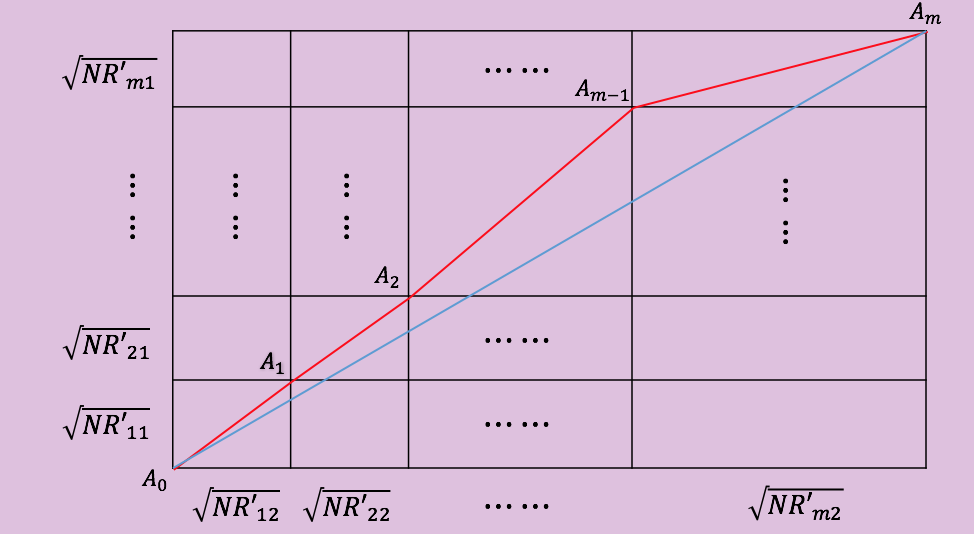
\includegraphics[width = 0.6\textwidth]{../common/m1.png}
   		 	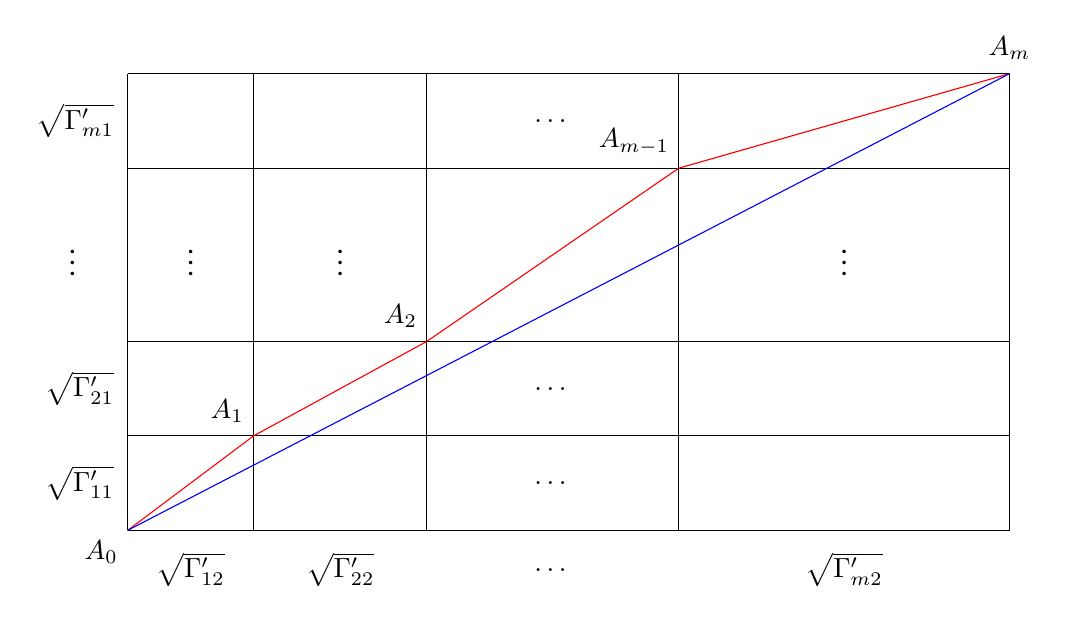
\begin{tikzpicture}
\pgfmathsetmacro{\HEIGHT}{1.2}
\pgfmathsetmacro{\HDOT}{2.2}
\pgfmathsetmacro{\WDOT}{3.2}
\pgfmathsetmacro{\WOne}{1.6}
\pgfmathsetmacro{\WTwo}{2.2}
\pgfmathsetmacro{\WN}{4.2}

\pgfmathsetmacro{\LEN}{\WOne + \WTwo + \WN + \WDOT}
\pgfmathsetmacro{\TH}{3*\HEIGHT+ \HDOT}

\tikzset{
  t/.style={draw, on grid, align=center, minimum height=1ex},
  coord/.style={coordinate, on grid, node distance=6mm and 25mm},
  between/.style args={#1 and #2}{
         at = ($(#1)!0.5!(#2)$)
    }
}

\draw [name path=h1] (0, 0) -- (\LEN, 0);
\draw [name path=h2] (0, \HEIGHT) -- (\LEN, \HEIGHT);
\draw [name path=h3] (0, 2*\HEIGHT) -- (\LEN, 2*\HEIGHT);
\draw [name path=h4] (0, 2*\HEIGHT + \HDOT) -- (\LEN, 2*\HEIGHT + \HDOT);
\draw [name path=h5] (0, 3*\HEIGHT + \HDOT) -- (\LEN, 3*\HEIGHT + \HDOT);

\draw[name path=v1] (0, 0) -- (0, \TH);
\draw[name path=v2] (\WOne, 0) -- (\WOne, \TH);
\draw[name path=v3] (\WOne + \WTwo, 0) -- (\WOne + \WTwo, \TH);
\draw[name path=v4] (\WOne + \WTwo + \WDOT, 0) -- (\WOne + \WTwo + \WDOT, \TH);
\draw[name path=v5] (\WOne + \WTwo + \WDOT + \WN, 0) -- (\WOne + \WTwo + \WDOT + \WN, \TH);

\path [name intersections={of=h1 and v1,by=A0}];
\path [name intersections={of=h2 and v2,by=A1}];
\path [name intersections={of=h3 and v3,by=A2}];
\path [name intersections={of=h4 and v4,by=Am1}];
\path [name intersections={of=h5 and v5,by=Am}];

\draw [red] (A0) -- (A1) -- (A2) -- (Am1) -- (Am);
\draw [blue] (A0) -- (Am);

\node [below=0.01 of A0, anchor=north east] {$A_0$};
\node [above=0.05 of A1, anchor=south east]{$A_1$};
\node [above=0.05 of A2, anchor=south east] {$A_2$};
\node [above=0.05 of Am1, anchor=south east] {$A_{m-1}$};
\node [above=0.05 of Am, anchor=south]{$A_m$};


\path [name intersections={of=h1 and v1,by=t00}];
\path [name intersections={of=h2 and v1,by=t01}];
\path [name intersections={of=h3 and v1,by=t02}];
\path [name intersections={of=h4 and v1,by=t03}];
\path [name intersections={of=h5 and v1,by=t04}];
\node [coord, between=t00 and t01] (x1){};
\node [coord, between=t01 and t02] (x2){};
\node [coord, between=t02 and t03] (x3){};
\node [coord, between=t03 and t04] (x4){};

\node [left=0.05 of x1.west] {$\sqrt{{\nr}'_{11}}$};
\node [left=0.05 of x2.west] {$\sqrt{{\nr}'_{21}}$};
\node [left=0.7 of x3.west, anchor=center] {$\vdots$};
\node [left=0.05 of x4.west] {$\sqrt{{\nr}'_{m1}}$};

\path [name intersections={of=h1 and v1,by=s00}];
\path [name intersections={of=h1 and v2,by=s01}];
\path [name intersections={of=h1 and v3,by=s02}];
\path [name intersections={of=h1 and v4,by=s03}];
\path [name intersections={of=h1 and v5,by=s04}];
\node [coord, between=s00 and s01] (y1){};
\node [coord, between=s01 and s02] (y2){};
\node [coord, between=s02 and s03] (y3){};
\node [coord, between=s03 and s04] (y4){};

\node [below=0.5 of y1.south, anchor=center] {$\sqrt{{\nr}'_{12}}$};
\node [below=0.5 of y2.south, anchor=center] {$\sqrt{{\nr}'_{22}}$};
\node [below=0.5 of y3.south, anchor=center] {$\dots$};
\node [below=0.5 of y4.south, anchor=center] {$\sqrt{{\nr}'_{m2}}$};

\node at (x1.east -| y3.north) {$\dots$};
\node at (x2.east -| y3.north) {$\dots$};
\node at (x4.east -| y3.north) {$\dots$};

\node at (y1.north |- x3.east) {$\vdots$};
\node at (y2.north |- x3.east) {$\vdots$};
\node at (y4.north |- x3.east) {$\vdots$};

\end{tikzpicture}

   		 	\caption{Proof by shortest distance\label{fig:path}}
   		 \end{figure}
   As shown in Figure~\ref{fig:path}, we construct a grid whose length and width are divided into $m$ segments,  the $i$-th segment of which has length $\sqrt{\nr'_{i1}}$ and $\sqrt{\nr'_{i2}}$ respectively. 
   
   	Then, $S_1^{'2}+S_2^{'2}=A_0A_m^2$, that is, equals to the square of the blue segment's length. In the meanwhile, 
   	 $$S_1^2 = (\sum_{i=1}^m \sqrt{\nr_{i1}})^2 > (\sum_{i=1}^m \sqrt{\nr'_{i1}+\nr'_{i2}})^2 = (\sum_{i=1}^m A_{i-1}A_i)^2$$,
   	 which equals to the sum of squares of all red segments. Since the shortest distance between two points is a line-segment, it holds that $S_1^2 >S_1^{'2}+S_2^{'2}$.
   	 
   	 For the cases where $k>2$ DApps are split, 	we can regard it as successive splits and iteratively use the result on $k=2$. 
   	 
   	 So the property is proved.
   	 
\end{proof}

\subsection{Proof of Corollary~\ref{c1}}
\label{subsection:proof3}
\begin{proof}
	For any voter that is bought over by $d_1$'s developer, before splitting, we can regard the voter as a normal voter who values all DApps with weight vector $(1,0,0,...,0)$, as he gives his all voting capacity to $d_1$. Suppose now $d_1$ is split into $k$ DApps and the bough-over voter's contributory values to the $k$ DApps are $\nr_{t1},...,\nr_{tk}$, whose sum is fixed. According to the condition that the equality holds for Cauthy's inequality in the proof of Property~\ref{p1}, the voter can be regard as a normal voter who values all DApps with weight vector $(\sqrt{\nr_{t1}}/C,\sqrt{\nr_{t2}}/C,...,\sqrt{\nr_{tk}}/C,0,0,...,0)$, where $C=\sum_{j=1}^k \sqrt{\nr_{tj}}$. That is, the voter values the split DApps with weights according to kind of proportion and values all other DApps with 0 weights.~\footnote{Note that scaling all weights by a constant does not effect the results, since the total contributory value of the voter only depends on the proportions of weights to total weights}. Since
		$$\sum_{j=1}^k \sqrt{\nr_{tj}}/C =1$$
	so the case in this corollary can be reduced to the case about normal voters(Property~\ref{p2}). So the corollary is proved.
\end{proof}

\subsection{Proof of Property~\ref{p3}}
\begin{proof}
	We first consider the case that a voter splits his account into two sub-accounts. We fix the actions of other voters. Let $c$ to be the original account and $a,b$ to be the split sun-accounts, $S,S'$ to be the ranking score of the DApp that the voter plans to vote before and after splitting respectively, $U,U'$ to be the final reward of the developer of the DApp that the voter plans to vote before and after splitting respectively. By definition, we have 
	$$S= \sqrt{\nr_c}+O,~~S'=\sqrt{\nr_a}+\sqrt{\nr_b}+O$$,
	where $O$ is the sum of contributory values by other voters, which is fixed. 
	
	By ~\ref{eq:sqrt_nr} it holds that $S < S'$. That is, the rank of the DApp does not increase. 
	
	In the meanwhile, by definition, 
	$$U = \frac{S}{S+P}\lambda M,~~U' = \frac{S'}{S'+P} \lambda M$$,
	where $P$ is the sum of squares of other DApp's ranking score, which is fixed. 
	
	Since $S < S'$ it holds that $U \leq U'$. That is the developer's final reward does not increase.
	
	For the cases where $k>2$ sub-accounts are split, we can regard it as successive splits and iteratively use the result on $k=2$. 
	
\end{proof}
%\section{Registro de cambios}
\subsection{2019.4.8 registro de cambios}
\begin{itemize}
	\item Se reemplaza la función de NR a capacities (\ref{eq:capacity}) mediante $f(\mathcal{C}(a_i))=\mathcal{C}(a_i)$
	\item Se reemplaza el cálculo del factor de participación $\lambda$ (\ref{eq:participation}) mediante $\min\{\frac{0.008}{1-r},1\}$, donde $r=\frac{\nr_p}{\nr_s}$
	\item Se corrigen errores de tipeo.
\end{itemize}
\end{appendices}

\end{document}

%%% Local Variables:
%%% mode: latex
%%% TeX-master: t
%%% End:
